\section{Datasets} \label{sec:datasets}
% TODO rewrite dataset chapter
% TODO look at overleaf comments for the dataset and metrics chapters

When using deep learning networks, it is important to choose a dataset (or multiple datasets) that optimally fulfills the requirements for its purpose. The dataset will be used to train and evaluate the deep learning network on. So, if the datasets is faulty, the resulting model will be faulty as well. A faulty model will predict faulty \glspl{OGM}, which could cause dangerous situations if it is used by an \gls{AV} and affects its decisions regarding motion planning. This chapter first discusses what the requirements are for a dataset that is used for \gls{OGM} prediction. Then, based on those requirements, nine criteria are devised that are used to evaluate the adequacy of a dataset. Subsequently, ten datasets are evaluated against the criteria and compared with one another. A dataset top 3 is presented in this chapter's conclusion in which the question \airquote{\textit{What dataset is most suitable to generate \gls{OGM} sequences for \gls{OGM} prediction?}} is answered. \\

In the case of \gls{OGM} prediction in a traffic scene context, a dataset is desired that contains \gls{BEV} environmental data of ego-vehicle centered traffic scenes that can be used to generate \gls{OGM} sequences. Moreover, if the dataset contains data that can be used to generate an extended form of the \gls{OGM}, as is discussed in chapter \ref{sec:ogm}, it would be beneficial. \\

It is important that the dataset's traffic scenes reflect the diversity of real world situations. The way a dataset's data is sampled from a population can influence how much the dataset reflects reality. A model that is trained on biased data could generate inaccurate predictions \cite{mehrabi2019survey}. If a traffic scene dataset is obtained in only one geographic, environmental, or cultural location, the dataset will contain some kind of bias towards the behavior, representation, and environmental context of that location \cite{mehrabi2019survey}. For example, \cite{nordfjaern2010investigation}'s research shows that geographical location (rural vs urban), and factors such as age, gender, and education influence the behavior of drivers. Also, \cite{nordfjaern2014culture} shows that traffic risk perception differs per culture and country. This can result in different traffic behavior between countries given the same traffic scene context. It is therefore important that a dataset contains data from multiple locations in varying geographical, cultural, and environmental areas. Also, the dataset should be diverse in the kind of traffic participants it contains. Besides vehicles and pedestrians, it is desired that the dataset contains other traffic participant classes (e.g. cyclists, riders). The more diverse the dataset is, the smaller the dataset bias is, and the better the prediction accuracy is of the model that is trained on that dataset. Besides having diverse data, the performance of a deep learning network also increases with a logarithmically increasing dataset size \cite{torralba2011unbiased}. Therefore, a dataset should be large besides being diverse. For large-scale datasets, even rare traffic cases are expected to be captured enough times so the deep learning network can generalize those situations accurately. \\

Regarding the traffic scene sequences, literature does not mention the ideal frame rate that \gls{OGM} sequences should have to generate optimal predictions, \cite{chen2007review} reviewed literature on what the influence of frame rate of visual perceptions is on human perceptual performance. In \cite{chen2007review}'s reviewed papers, humans are situated in virtual environments in which the visual information of the environment is updated at a variable frame rate. The research shows that higher frame rates increase the performance (accuracy, reaction time, recognition) at which humans completed certain perceptual tasks. Frame rates below 10 Hz showed sharp performance degradations, while frame rates higher than 15 Hz did not increase performance significantly. Therefore, a frame rate of 10 Hz is considered the minimum threshold for accurate human perceptual understanding. Using humans as reference for the performance of deep learning networks, a frame rate of 10 Hz is also considered as the minimal threshold for accurate \gls{OGM} prediction. So, it is desired that a dataset has at least a 10 Hz sampling rate of its environment. Furthermore, the traffic scene sequences should be long enough. The sequences have to be split into a part that represents the 'past' to use as input sequences for the deep learning network, and a ground truth of the 'future' to compare the predictions with. The research by \cite{lange2020attention} uses $0.5$s of past \glspl{OGM} to predict up to $1.5$s of future \glspl{OGM}. So, a sequence of $2$s is sufficient to perform \gls{OGM} prediction using this method. If a margin of $0.5$s is considered for the length of the past information and for the length of the prediction horizon, a dataset should provide \gls{OGM} sequences of at least $3$s long. \\

Aside from the contents of the dataset, the quality of the sensors with which the dataset is recorded is essential. The resolutions of the sensors should be high enough to capture the smallest traffic participant's (\glspl{VRU}) behavioral patterns. Not only the performance of deep learning network, but also the time that is required to pre-process, train, and evaluate the network is greatly dependent on what dataset is used. Also, the performance of a network should be compared reliably. Therefore, it is important that a dataset is chosen on which other research has based their network training and evaluation on, so there are enough results for reliable comparisons. \\

To ensure that the optimal dataset is chosen for \gls{OGM} prediction research, the following list of criteria is devised which a dataset has to meet in order to be suitable for \gls{OGM} prediction. The criteria are based on the  Based on how the dataset scores on this list, an informed decision can be made. 

\begin{enumerate}
	\item The dataset contains data of ego-vehicle centered traffic scene sequences that provide at least 2D \gls{BEV} information of the environment.
	\item The dataset provides enough diverse data to train and evaluate a network on.
	\item The dataset contains traffic scene sequences, or provides means to easily generate them.
	\item The sequences have enough frames per sequence and a frame rate that is suitable for capturing road user behavior and trajectories.
	\item The sequences contain various traffic actors including vehicles and \glspl{VRU}.
	\item The dataset data, and any \gls{OGM} that can be generated from it, provides a resolution that is high enough to distinguish and to track \glspl{VRU}. 	
	\item The sequences show a diversity in environmental properties, containing \glspl{VRU}, that may influence the generated \glspl{OGM} (e.g. urban vs rural, dense vs sparse traffic).
	\item The dataset provides data, including ground truth, that is required for generating extended \gls{OGM} forms.
	\item Results of other research using the dataset for generating and predicting \glspl{OGM} is available for comparison. 
\end{enumerate}


A total of ten datasets coming from three categories are found that contain ego-vehicle centered traffic scene sequences. Three datasets were created for a purpose that includes motion prediction. Five datasets were created for object detection purposes. The last two datasets were mainly created to research semantic segmentation on. All the datasets are recorded using a vehicle equipped with one or multiple sensors that drives through real traffic. \\

To evaluate the datasets against the criteria, information about each dataset is gathered and put into a table (see table \ref{tab:datasets_overview}). The first criterion is met if the dataset contains 2D \gls{BEV} information about the environment. From the recording vehicle's point of view, having 2D \gls{BEV} information means that the vehicle should gather 3D sensor data which can be projected onto the 2D top view plane. The information about the sensors provides the data to evaluate this first criterion. The second criterion is tested using information about the number of categories and classes that are labelled in the datasets. If the dataset contains sequences of its sensor data, the third criterion is met. The fourth criterion is tested by evaluating the sampling frequency and length of the sequences. To test the fifth criterion, the number (and presence) of vehicles and pedestrians is evaluated. The information about the sensors is used to test the sixth criterion. The seventh criterion is evaluated by examining the diversity of sampling locations. Then, the eighth criterion is met if the dataset contains data to generate extended \glspl{OGM}. Finally, the ninth criterion is tested by evaluating whether there exists literature that generates \glspl{OGM} from the dataset and whether there is literature that uses those generated \glspl{OGM} for \gls{OGM} prediction. The evaluation and comparison of each dataset against the criteria is shown in table \ref{tab:datasets_criteria}. \\

The most interesting characteristics of each dataset are highlighted below in three subsections based on the dataset's original purposes: Motion prediction (section \ref{subsec:data_track_mot}), Object Detection (section \ref{subsec:data_ob_det}), and Semantic Segmentation (section \ref{subsec:data_sem_seg}). At the end of this chapter (section \ref{subsec:data_con}) a conclusion about the datasets is provided.


\subsection{Tracking and Motion prediction Datasets} \label{subsec:data_track_mot}
The following three datasets are obtained for tracking or motion prediction purposes. The \gls{STIP} dataset \cite{liu2020spatiotemporal}, the Argoverse dataset \cite{chang2019argoverse} and the RoboCar dataset \cite{robotcardatasetijrr}. \\

The \gls{STIP} dataset \cite{liu2020spatiotemporal} is obtained using three cameras (left, front and right) with a 1216x1936 resolution at 20 Hz positioned on the recording vehicle. An example of the \gls{STIP} dataset's camera images is shown in figure \ref{fig:dat_stip}. However, these are not stereo cameras, so no 3D information is obtained. This dataset does therefore not meet the first criterion. 3D information can be computed from the monocular images using monocular unsupervised depth estimation techniques \cite{godard2017unsupervised}. However, this probably will not yield as reliable results compared to stereo vision data and the time spent on generating 3D data could also be spent on training a network using a dataset that does contain 2D \gls{BEV} information. A remarkable property of this dataset is that the sampling frequency of the camera images is 20 Hz. When comparing the \gls{STIP} dataset's sampling rate to the other dataset's rates (see table \ref{tab:datasets_overview}, it can be seen that this dataset, together with the \gls{ECP2.5D} \cite{braun2020ecp2} dataset has the highest sampling rate. \\

\begin{figure}[h!]
	\centering
	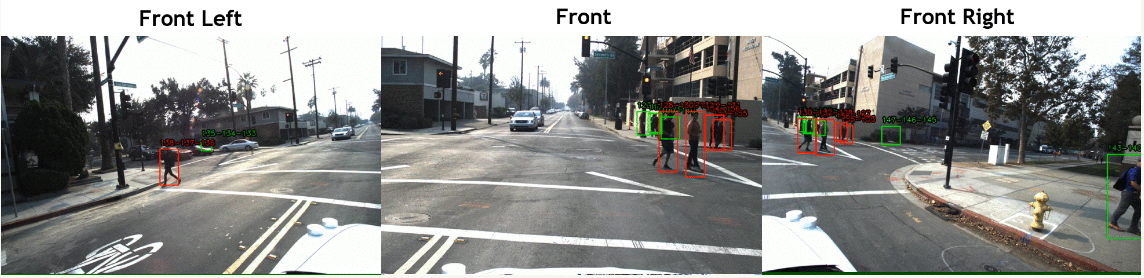
\includegraphics[width=0.8\linewidth]{Figures/Datasets/STIP_Dataset}
	\caption{This image shows an overview of the \gls{STIP} \cite{liu2020spatiotemporal} dataset's camera images. Pedestrians are annotated with cross (red) not-cross (green) labels.  \cite{liu2020spatiotemporal}}  
	\label{fig:dat_stip}
\end{figure}

The Argoverse dataset \cite{chang2019argoverse} is recorded in only two cities in one country. It therefore contains little geographic diversity compared to the \gls{ECP2.5D} \cite{braun2020ecp2} and Cityscapes \cite{cordts2016cityscapes} datasets. On the other side, the Argoverse dataset \cite{chang2019argoverse} contains 333K 5-second sequences and labels 17 different classes, including vehicles, pedestrians and cyclists. Furthermore, \cite{roddick2020predicting} has already used this dataset to generate \glspl{OGM}. Examining \cite{roddick2020predicting}'s research could therefore speed up the \gls{OGM} generation time. \\

The RoboCar dataset \cite{robotcardatasetijrr} is collected in only one city and no data is labeled. It is therefore not a diverse dataset compared to the other datasets. The dataset contains 360-second sequences, but of an unkown number. What is beneficial about this dataset is that \cite{dequaire2018deep} and \cite{wang2020l2r} used it for \gls{OGM} generation before, where \cite{dequaire2018deep} also performed \gls{OGM} prediction.


\subsection{Object Detection Datasets} \label{subsec:data_ob_det}
This subsection will discuss five datasets that were originally obtained for object detection purposes. The \gls{ECP2.5D} dataset \cite{braun2020ecp2}, the \gls{BDD100K} dataset \cite{yu2020bdd100k}, the \gls{KITTI} dataset \cite{geiger2012we}, the nuScenes dataset \cite{caesar2020nuscenes}, and the Waymo Open dataset \cite{sun2020scalability}. \\

The \gls{ECP2.5D} dataset \cite{braun2020ecp2} contains 15-second sequences in which seven different classes are labeled. This is average compared to the other datasets. This dataset is remarkable because it is recorded in 31 cities in 12 countries which makes this the most diverse datatset regarding geographic locations. Also, the sampling frequency of the sequences is 20 Hz, which is the highest together with the \gls{STIP} dataset \cite{liu2020spatiotemporal}. An example of the camera and LiDAR data of the \gls{ECP2.5D} dataset \cite{braun2020ecp2} is shown in figure \ref{fig:dat_ecp}. \\

\begin{figure}[h!]
	\centering
	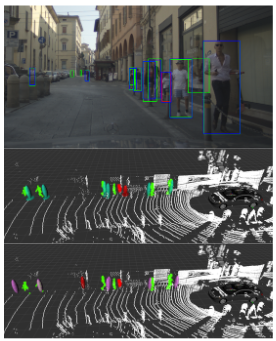
\includegraphics[width=0.4\linewidth]{Figures/Datasets/ECP_Dataset}
	\caption{This image shows an example of how the \gls{ECP2.5D} \cite{braun2020ecp2} dataset contains camera and LiDAR data in which pedestrians are annotated.}  
	\label{fig:dat_ecp}
\end{figure}

The \gls{BDD100K} dataset \cite{yu2020bdd100k} is collected using crowd-sourcing. Drivers could upload their data obtained by using a 1280x720 resolution front camera at 30 Hz together with GPS/IMU localization data. Recordings were mostly made in San Francisco and the Bay Area, New York, and Berkeley which makes it average on geographic diversity. Because of the crowd-sourcing, large amounts of data could be obtained. The dataset contains 100K 40-second sequences which makes it one of the largest datasets compared to the other datasets. Moreover, the dataset contains pixel-level semantic segmentation of the vehicle's drivable area. A downside of this dataset is that it is obtained using solely a monocular camera. Therefore, some unsupervised depth estimation technique must be performed to gather 3D data, like the \gls{STIP} dataset \cite{liu2020spatiotemporal}. \\

The \gls{KITTI} dataset \cite{geiger2012we} is the smallest dataset (of which the number of sequences is known) compared to the other datasets. It only contains 22 sequences and is obtained in only one country. The benefit of using this dataset is that it has been used by \cite{itkina2019dynamic}, \cite{mohajerin2019multi}, and \cite{lange2020attention} to generate and predict \glspl{OGM}. So, there is enough research to compare prediction methods with that use the \gls{KITTI} dataset \cite{geiger2012we}. \\

For the nuScenes dataset \cite{caesar2020nuscenes}, a LiDAR that can generate a 1.4M point 360 degree view at 20 Hz, five radars around the vehicle with a 250m range at 13 Hz, and six 1600x900 resolution cameras around the vehicle at 12 Hz are used to collect data. However, the sampling frequency of the data is only 2 Hz. This is the lowest sampling frequency compared to other datasets. Figure \ref{fig:dat_nuscenes} shows an example of the six camera images overlayed with the LiDAR point cloud of the nuScenes dataset \cite{caesar2020nuscenes}. The advantage of this dataset is that it contains velocity information from the radar data. Besides that, the nuScenes dataset is collected for object detection as well as object tracking. Therefore, it contains 1000 sequences of 20 seconds. Objects of 23 classes are annotated, including vehicles, pedestrians, and riders. So, the nuScenes dataset \cite{caesar2020nuscenes} is larger and more diverse than most other datasets. The nuScenes paper \cite{caesar2020nuscenes} compares its dataset against the \gls{KITTI} dataset \cite{geiger2012we}. It concludes that training on the \gls{KITTI} dataset, with its smaller size compared to nuScenes, affects a network's performance. \\

\begin{figure}[h!]
	\centering
	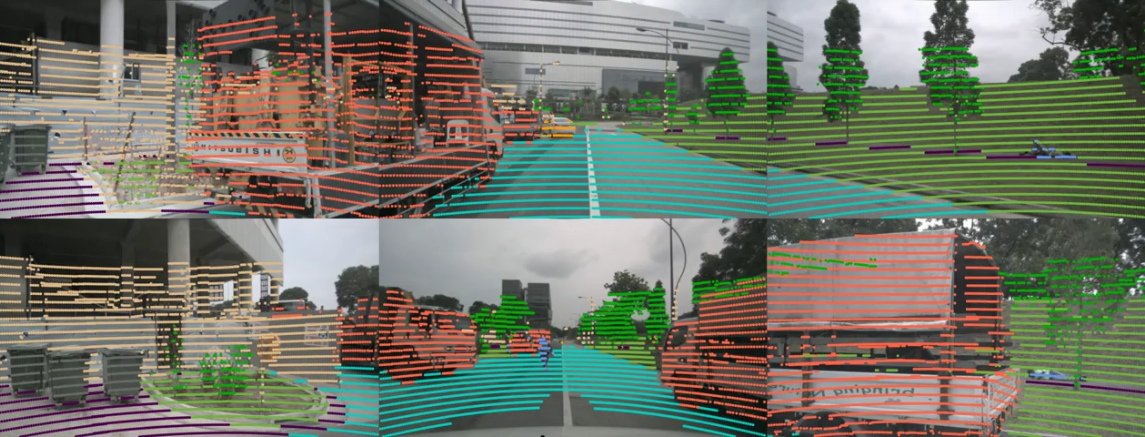
\includegraphics[width=0.6\linewidth]{Figures/Datasets/NuScenes_Dataset}
	\caption{This image shows an example of the images of the six cameras from the nuScenes dataset \cite{caesar2020nuscenes}. The images are overlayed with the semantic segmented LiDAR data.}  
	\label{fig:dat_nuscenes}
\end{figure}

The Waymo Open dataset \cite{sun2020scalability} (in short Waymo), was originally recorded in 3 cities (Phoenix, San Francisco, and Mountain View) and later extended with another 3 cities (Los Angeles, Detroit, and Seattle). This makes the dataset average on geographic diversity. Besides object detection, the Waymo dataset \cite{sun2020scalability} also focuses on data for motion prediction. It now contains 103K 20 second sequences at 10 Hz (together over 20M frames and 574 hours of data). It contains 10.8M objects with tracking IDs, labels for three object classes (vehicles, pedestrians, and cyclist), and 3D bounding boxes of each of those objects. Each sequence contains 3D map data and is further broken down into 9 second windows (1 second of historic frames and 8 seconds of future frames) with 5 second overlap for motion prediction purposes. This makes the dataset one of the largest datasets. Moreover, \cite{lange2020attention} and \cite{toyungyernsub2020double} used the Waymo dataset to generate and predict \glspl{OGM}, so there is research to compare prediction methods with using the Waymo dataset \cite{sun2020scalability}.


\subsection{Semantic Segmentation Datasets} \label{subsec:data_sem_seg}
This section discusses two datasets that are originally generated for semantic segementation tasks. The Apolloscape dataset \cite{huang2019apolloscape}  and the Cityscapes dataset \cite{cordts2016cityscapes}. \\

Apolloscape \cite{huang2019apolloscape} is a dataset which is collected for the purpose of scene parsing (semantic segmentation on pixel-level). Therefore, the dataset contains almost 144K frames with pixel-level annotations for semantic segmentation. Furthermore, 89K instance-level annotations are provided for movable objects. 25 different labels are annotated covering five groups. Also, 28 lane markings are annotated. Together there are 543K pedestrian instances and 1.99M vehicle instances in the dataset. This makes the dataset diverse regarding traffic participants. The downside is that the dataset is recorded in only one city, and there is no information available about presence of sequences (only individual frames). \\

\begin{figure}[h!]
	\centering
	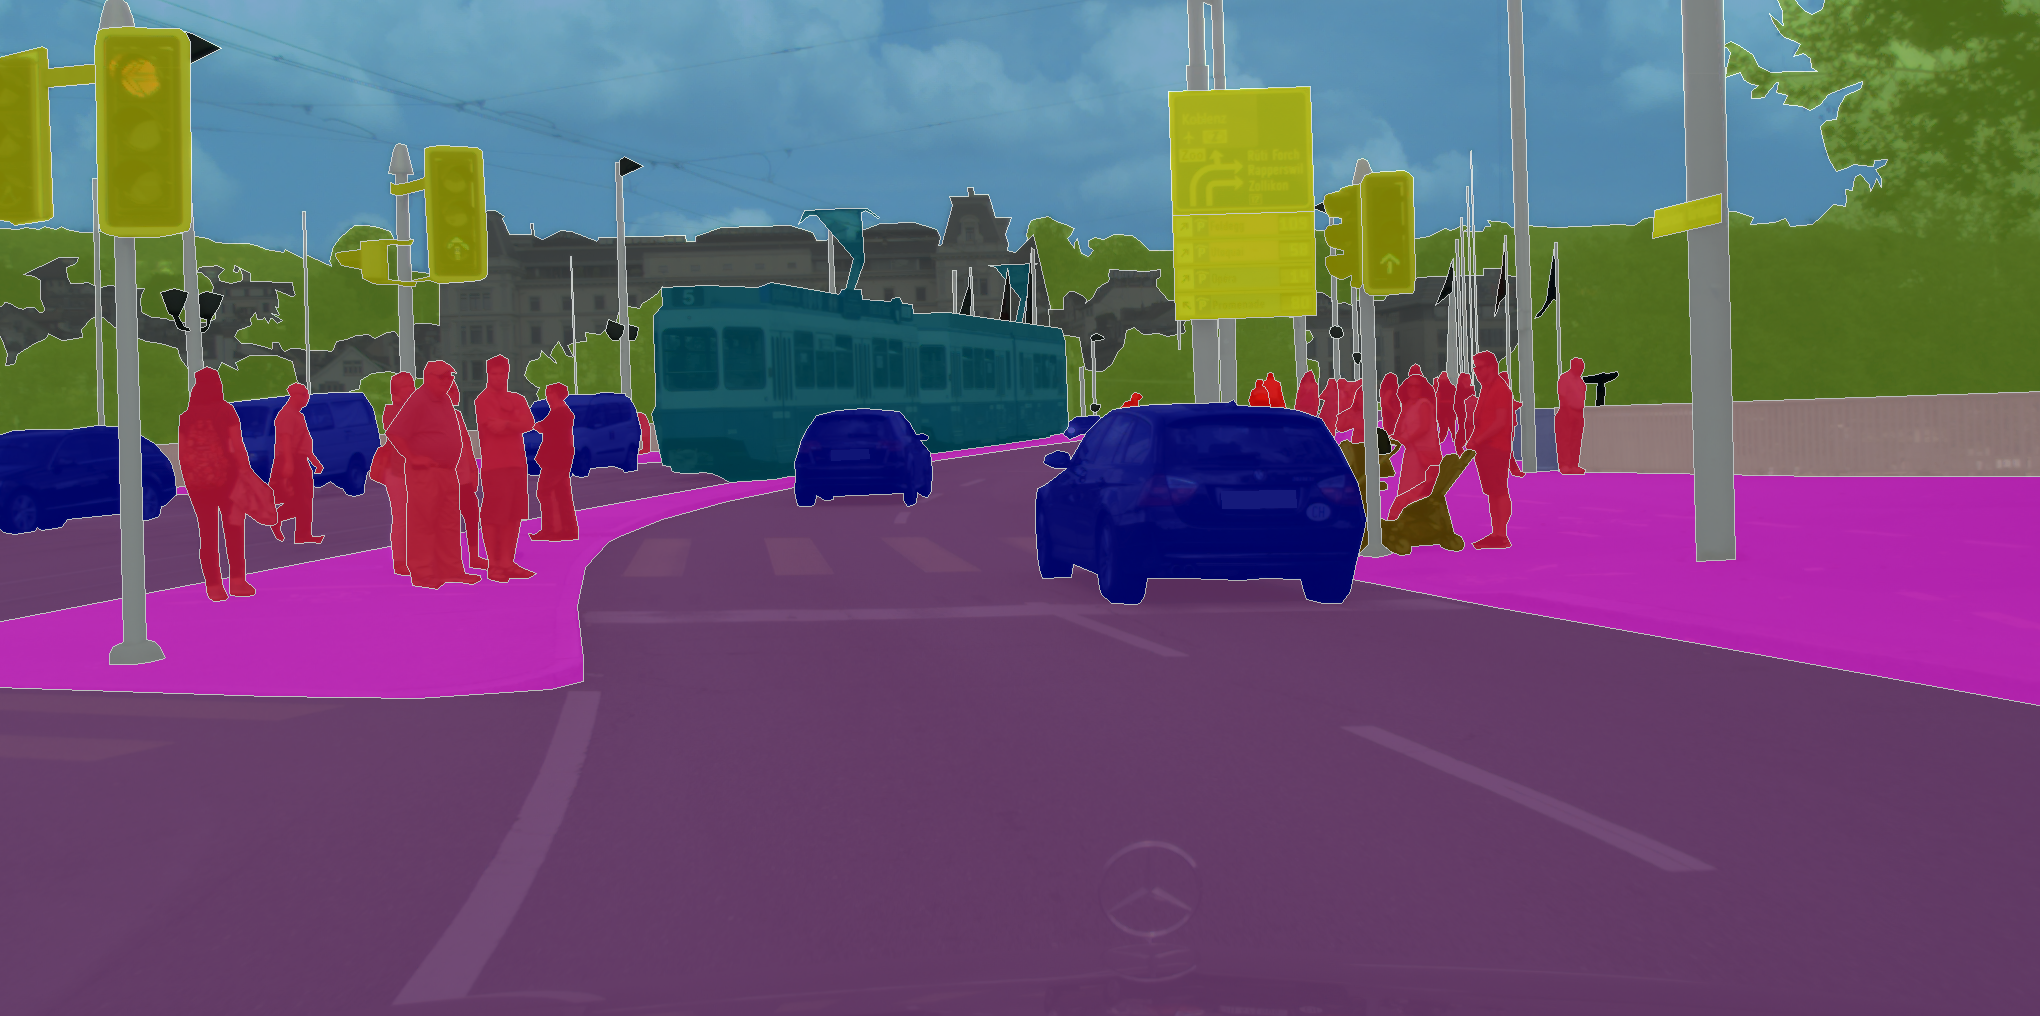
\includegraphics[width=0.6\linewidth]{Figures/Datasets/Cityscapes_Dataset}
	\caption{This image shows an example of the Cityscapes \cite{cordts2016cityscapes} dataset. The camera image is semantically segmented. Each object class in the image is given a different label (color).}  
	\label{fig:dat_cityscapes}
\end{figure}

The Cityscapes dataset \cite{cordts2016cityscapes} is recorded in 50 different cities, primarily in Germany but also in neighboring countries. From 27 cities, 5000 images are selected for dense pixel-level annotation. Annotations are done on every 20th frame of a 30-frame video sequence. For the remaining 23 cities, coarse annotation is performed on a single image every 20 seconds or 20 meters driving distance (whichever comes first). This yields another 20K annotated images. An example an annotated image from the dataset is shown in figure \ref{fig:dat_cityscapes}. 30 classes are annotated which are grouped into 8 categories. The dataset contains 24.4K annotated pedestrians and 41K vehicles. Humans and vehicles are also annotated on an instance level. Therefore, this dataset is diverse regarding both geographic locations and traffic participants. The dataset has also been used to generate \glspl{OGM} by \cite{hehn2021fast}. The downside of this dataset is that the number of sequences is not known, besides that it is a 'large set'. 

\subsection{What dataset is most suitable to generate \gls{OGM} sequences for \gls{OGM} prediction?} \label{subsec:data_con}

Table \ref{tab:datasets_overview} shows an overview of the datasets that are discussed in the previous subsections. Based on the properties of each dataset it is evaluated how well they meet the criteria that were set at the beginning of this chapter. If a criterion is met, the score of the dataset goes up by 1 point. If the criterion is met partially, or in average quality compared to the other datasets, the score goes up by 0.5 point. If a criterion is not met, or if it is met in a bad quality compared to other datasets, the dataset will not get any points for that criterion. Also, if information about a criterion is not found or not available, no points are given to the criterion. Table \ref{tab:datasets_criteria} shows an overview of how well each datasets scores per criterion. More information about the symbols and what score is linked to them is written below the table. \\

\begin{figure}[h]
	\centering
	\begin{subfigure}[t]{0.4\linewidth}
		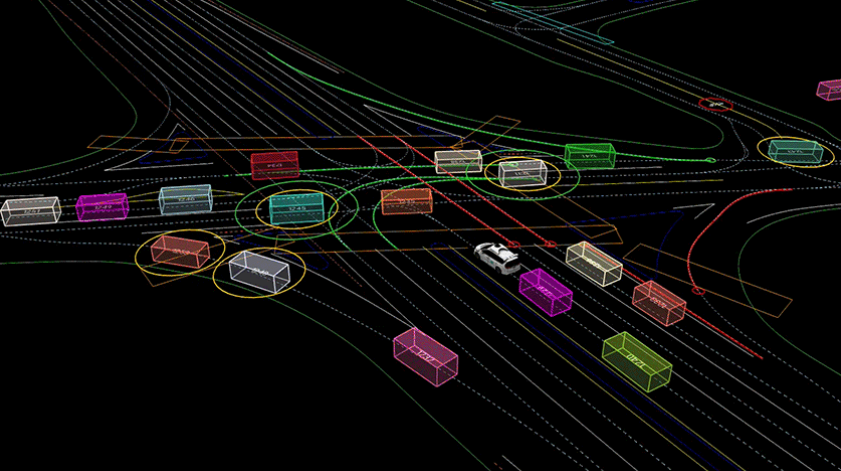
\includegraphics[width=\linewidth]{Figures/Datasets/Waymo_Dataset}
		\caption{This image shows an overview of the labeled vehicles and lane markings of the Waymo \cite{sun2020scalability} dataset.}
		\label{fig:dat_waymo_1}
	\end{subfigure} \hspace{0.1\textwidth}
	\begin{subfigure}[t]{0.4\linewidth}
		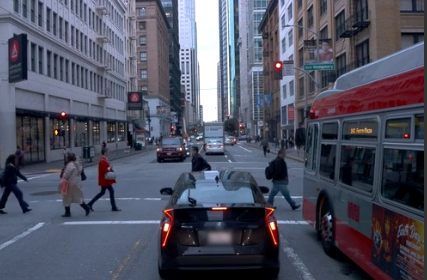
\includegraphics[width=\linewidth]{Figures/Datasets/Waymo_Dataset2}
		\caption{This image shows a front camera image of the Waymo \cite{sun2020scalability} dataset.}
		\label{fig:dat_waymo_2}
	\end{subfigure}
	\caption{Two examples of the Waymo \cite{sun2020scalability} dataset.}
	\label{fig:dat_waymo_both}
\end{figure}

With a score of 7.5, the Waymo \cite{sun2020scalability} dataset (shown in figure \ref{fig:dat_waymo_both}) is the most suitable dataset to generate \gls{OGM} sequences for \gls{OGM} prediction. While the diversity of the Waymo dataset is average, compared to the other datasets, and there is no (available) data to extend the \gls{OGM} form, the Waymo dataset meets all other criteria in good quality which sums up to the score of 7.5. Other suitable datasets on the second and shared third places are the Cityscapes \cite{cordts2016cityscapes}, Argoverse \cite{chang2019argoverse} and NuScenes \cite{caesar2020nuscenes} datasets with a score of 7.0, 6.5 and 6.5 respectively. Unlike the Waymo dataset, the Cityscapes dataset provides pixel-level semantic segmentation data and the Nuscenes dataset provides velocity data and semantic LiDAR data. In the case this additional data is desired for research on a specific \gls{OGM} prediction method, the Cityscapes or Nuscenes datasets can be more suitable to use than the Waymo dataset. Also, conveniently, for the four best scoring datasets there is literature available that provides code to generate \glspl{OGM} from the data. These sources can be found in table \ref{tab:datasets_overview}.  

\begin{table}[h!]
	\centering
	\resizebox{\linewidth}{!}{%
		\begin{tabular}{lllllllllll} 
			\toprule
			& \textbf{STIP \cite{liu2020spatiotemporal}} & \textbf{Argoverse \cite{chang2019argoverse}} & \textbf{ECP2.5D \cite{braun2020ecp2}} & \textbf{BDDK100 \cite{yu2020bdd100k}} & \textbf{KITTI \cite{geiger2012we}} & \textbf{NuScenes \cite{caesar2020nuscenes}} & \textbf{Waymo \cite{sun2020scalability}} & \textbf{Apolloscape \cite{huang2019apolloscape}} & \textbf{Cityscapes \cite{cordts2016cityscapes}} & \textbf{RoboCar \cite{robotcardatasetijrr}} \\ 
			\hline
			\textbf{1} & \xmark & \cmark & \cmark & \xmark & \cmark & \cmark & \cmark & \cmark & \cmark & \cmark \\
			\textbf{2} & \textbf{$\pm$} & \textbf{$\pm$} & \textbf{$\pm$} & \textbf{+} & \textbf{$-$} & \textbf{$\pm$} & \textbf{$\pm$} & \textbf{$-$} & \textbf{+} & \textbf{$-$} \\
			\textbf{3} & \textbf{$\pm$} & \textbf{+} & \textbf{$\pm$} & \textbf{+} & \textbf{$-$} & \textbf{+} & \textbf{+} & U & U & U \\
			\textbf{4} & \textbf{+} & \textbf{+} & \textbf{+} & U & \textbf{+} & \textbf{$-$} & \textbf{+} & U & \textbf{+} & \textbf{+} \\
			\textbf{5} & \cmark & \cmark & \cmark & \cmark & \cmark & \cmark & \cmark & \cmark & \cmark & U \\
			\textbf{6} & \cmark & \cmark & \cmark & \cmark & \cmark & \cmark & \cmark & \cmark & \cmark & \cmark \\
			\textbf{7} & \textbf{$\pm$} & \textbf{$\pm$} & \textbf{$\pm$} & \textbf{$\pm$} & \textbf{$\pm$} & \textbf{$\pm$} & \textbf{+} & \textbf{$\pm$} & \textbf{$\pm$} & \textbf{$\pm$} \\
			\textbf{8} & N & N & N & Pixel Semantics & N & Velocity data, LiDAR Semantics & N & Pixel Semantics & Pixel Semantics & N \\
			\textbf{9} & N & Only OGM gen & N & N & OGM gen and pred & Only OGM gen & OGM gen and pred & N & Only OGM gen & OGM gen and pred \\
			\textbf{Scores} & 4.5 & \textbf{6.5} & 5.5 & 5.5 & 5.5 & \textbf{6.5} & \textbf{7.5} & 4.5 & \textbf{7.0} & 4.5 \\
			\bottomrule
		\end{tabular}
	}
	\caption{
		The table shows for each dataset how well it scores per criterion. The scores are based on the information in table \ref{tab:datasets_overview}. The following symbols are used to evaluate each criterion: 
		\textbf{+:} Good, \textbf{$\pm$:} Average, \textbf{$-$:} Bad, \textbf{U:} Unknown: \textbf{N:} None/Not available/Not found, \textbf{\cmark:} Yes, \textbf{\xmark:} No. \\\hspace{\textwidth} 
		At the bottom row, each dataset is given a score based on which symbol is given at the evaluation, and whether there is useful information found for criteria 8 and 9. A '\textbf{+}', a '\textbf{\cmark}', 'OGM gen and pred', and any available additional data for an extended OGM form provide 1 point, an '\textbf{$\pm$}' and 'only OGM gen' provides 0.5 points, and the '\textbf{\xmark}', '\textbf{$-$}', 'U', and 'N' provide 0 points.  
		Below is the list of criteria. \\\hspace{\textwidth} 	
		\textbf{1.} The dataset contains data of ego-vehicle centered traffic scene sequences that provide at least 2D \gls{BEV} information of the environment.
		\textbf{2.} The dataset provides enough diverse data to train and evaluate a network on.
		\textbf{3.} The dataset contains traffic scene sequences, or provides means to easily generate them.
		\textbf{4.} The sequences have enough frames per sequence and a frame frequency that is suitable for capturing road user behavior and trajectories.
		\textbf{5.} The sequences contain various traffic actors including vehicles and \glspl{VRU}.
		\textbf{6.} The dataset data, and any \glspl{OGM} that can be generated from it, provides a resolution that is high enough to distinguish and to track \glspl{VRU}. 
		\textbf{7.} The sequences show a diversity in environmental properties, containing \glspl{VRU}, that may influence the generated \glspl{OGM} (e.g. urban vs rural, dense vs sparse traffic).
		\textbf{8.} The dataset provides data, including ground truth, that is required for generating extended \gls{OGM} forms.
		\textbf{9.} Results of other research using the dataset for generating and predicting \glspl{OGM} is available for comparison.}
	\label{tab:datasets_criteria}
\end{table}


\afterpage{%
	\clearpage% Flush earlier floats (otherwise order might not be correct)
	\thispagestyle{empty}% empty page style (?)
	\begin{landscape}
		\begin{longtable}{m{4em}m{2em}m{7em}m{7em}m{5em}m{2em}m{5em}m{7em}m{4em}m{2em}m{2em}m{5em}m{1em}m{1em}} 
			\toprule
			\rotatebox{90}{\textbf{Dataset}} & \rotatebox{90}{\textbf{Year}} & \multicolumn{3}{c}{\rotatebox{90}{\textbf{Sensors}}} & \rotatebox{90}{\textbf{Sampling Frequency}} & \rotatebox{90}{\textbf{Diversity of Locations}} & \rotatebox{90}{\textbf{Dataset size}} & \rotatebox{90}{\textbf{Diversity of labels}} & \rotatebox{90}{\textbf{\# Pedestrians}} & \rotatebox{90}{\textbf{\# Vehicles}} & \rotatebox{90}{\textbf{Extended OGMs}} & \rotatebox{90}{\textbf{OGM generation method}} & \rotatebox{90}{\textbf{OGM prediction comparison}} \endfirsthead
			\midrule
			\textbf{STIP \cite{liu2020spatiotemporal}} & 2020 & - & 3 RGB cameras of res 1216x1936  (20 Hz) & - & 20 Hz & 1 country, 8 cities, dense urban areas & 556 sequences, \textasciitilde{}2h of recording, \textasciitilde{}150K frames & 2 classes (pedestrian, vehicle) & \textasciitilde{}3K & - & - & - & - \\
			\textbf{Argoverse \cite{chang2019argoverse}} & 2019 & 2 VLP-32 LiDARs with 200m range (10 Hz) & 7 RGB cameras in 360 deg setup of res 1920x1200 (30 Hz) and 2 in stereo view of res  2056x2464 (5 Hz) & GPS/ Odometry sensor & 10 Hz & 1 country, 2 cities, dense urban areas & \textasciitilde{}333K 5s sequences, 1006h of recording, spanning \textasciitilde{}290km & 17 classes & \textasciitilde{}1.5K & \textasciitilde{}8K & - & \cite{roddick2020predicting} & - \\
			\textbf{ECP2.5D \cite{braun2020ecp2}} & 2020 & Velodyne HDL-64E LiDAR with 120m range (5-20 Hz) & 1 RGB camera of res 1920x1024 (20 Hz) & GPS/INS & 20 Hz & 12 countries, 31 cities, dense urban areas & 15s sequences, 46K frames & 7 classes & \textasciitilde{}218K & - & - & - & - \\
			\textbf{BDDK100 \cite{yu2020bdd100k}} & 2020 & - & 1 camera of res 1280x720 (30 Hz) & GPS/IMU & - & (mostly) 1 country, 4 cities, dense urban areas & \textasciitilde{}100K 40s sequences & 3 categories, 20 classes & \textasciitilde{}129K & \textasciitilde{}1M & Pixel-level semantic segmentation & - & - \\
			\textbf{KITTI \cite{geiger2012we}} & 2012 & Velodyne HDL-64 LiDAR with 100m range (10 Hz) & 4 cameras (2 color 2 grayscale) of res 1392x512 (10 Hz) & GPS/IMU & 10 Hz & 1 country, 1 city, dense urban areas & 22 sequences & 2 categories, 8 classes & \textasciitilde{}9.4K & \textasciitilde{}100K & - & \cite{itkina2019dynamic} \cite{mohajerin2019multi} \cite{lange2020attention} & \cite{itkina2019dynamic} \cite{mohajerin2019multi} \cite{lange2020attention} \\
			\textbf{NuScenes \cite{caesar2020nuscenes}} & 2019 & 32 beam LiDAR 1.4M points/s (20 Hz) + 5 Radars with 250m range (13 Hz) & 6 cameras of res 1600x900 cameras (12 Hz) & GPS/IMU, CAN bus data & 2 Hz & 2 countries, 2 cities, dense urban areas & 1000 20s sequences & 23 classes, 8 attributes & \textasciitilde{}200K & \textasciitilde{}500K & velocity information from Radar with 0.1km/h accuracy and LiDAR semantics & \cite{roddick2020predicting} \cite{loukkal2021driving} & - \\
			\textbf{Waymo \cite{sun2020scalability}} & 2020 & 5 LiDAR sensors (1 mid range, 4 short range) & 5 cameras (3 front of res 1920x1280 and 2 side of res 1920x1014) & - & 10 Hz & 1 country, 6 cities, urban and suburban areas & 103K 20s sequences & 3 classes & \textasciitilde{}2.8M & \textasciitilde{}6.1M & - & \cite{lange2020attention} \cite{toyungyernsub2020double} & \cite{lange2020attention} \cite{toyungyernsub2020double} \\
			\textbf{Apolloscape \cite{huang2019apolloscape}} & 2018 & 2 VUX-1HA LiDARs with 420m range & 1 VMX-CS6 camera system with 2 cameras of res 3384x2710 (no depth information) & IMU/GNSS & - & 1 country, dense urban areas & - & 5 categories, 35 classes, additional 28 kinds of lane markings & \textasciitilde{}543K & \textasciitilde{}1.99M & Pixel-level semantic segmentation & - & - \\
			\textbf{Cityscapes \cite{cordts2016cityscapes}} & 2020 & - & 1 stereo camera of res 1920x1080 (OnSemi AR0331) (17 Hz) & GPS, outside temperature, in-vehicle odometry sensors & 17 Hz & 1 country, 50 cities, dense urban areas & A 'large set' of sequences & 8 categories, 30 classes & \textasciitilde{}24.4K & \textasciitilde{}41K & Pixel-level semantic segmentation & \cite{hehn2021fast} & - \\
			\textbf{RoboCar \cite{robotcardatasetijrr}} & 2016 & 2 SICK LMS-151 2D LiDARs with 50m range (50 Hz) and 1 SICK LD-MRS 3D LiDAR with 50m range (12.5 Hz) & 4 cameras (1 front of res 1280x960 at 16 Hz, 3 for sides and rear of res 1024x1024 at 11.1 Hz) & GPS/INS & - & 1 country, 1 city, urban area & 360s sequences of unknown amount & No labels & - & - & - & \cite{dequaire2018deep} \cite{wang2020l2r} & \cite{dequaire2018deep} \\
			\bottomrule
		\caption{This table shows an overview of the datasets that are most likely to be suitable for \gls{OGM} prediction purposes.}
		\label{tab:datasets_overview}	
		\end{longtable}	
	\end{landscape}
}

%%



\newpage

\section{Metrics} \label{sec:metrics}

\glspl{AV} can have collision avoidance systems that make use of traffic scene predictions to estimate whether the ego-vehicle will collide with any of the surrounding traffic participants. Based on these systems the \gls{AV} can make decisions to drive as safe as possible by preventing or mitigating collisions. For example, if a collision is predicted, the ego-vehicle can decide to adjust its velocity to prevent or mitigate the collision, or it will decide to perform an evasive maneuver \cite{annell2016probabilistic} \cite{wang2019crash}. \cite{annell2016probabilistic}'s system has even shown to be robust to noise in the environment representation. However, due to prediction errors, such as artifacts or displacement errors of traffic participants, the \gls{AV} might make the wrong decisions (e.g. perform an evasive maneuver when in reality there is no imminent collision, or fail to perform an evasive maneuver when there is actually a collision risk). This can be dangerous for the \gls{AV} and its surroundings. Besides for the task of collision avoidance, prediction of an \gls{AV}'s surroundings can also improve the efficiency and safety of motion planning by \glspl{AV} in general. Ensuring safe motion planning means that no (additional) dangerous situations are caused when the \gls{AV} executes a path that is planned in the \gls{OGM} predictions, compared to a path that is planned in the ground truth \gls{OGM}. So, for the safety of \glspl{AV} and its surroundings, good predictions are important. Since this literature study focuses on \gls{OGM} predictions, a metric is desired that compares the predicted \glspl{OGM} with the ground truth \glspl{OGM}. \\

The quantitative evaluation of \gls{OGM} prediction methods depends highly on what metric is used to assess a method's performance. The metric determines which errors are considered and how much they weigh in the evaluation. What the best metric is for \gls{OGM} prediction is therefore investigated in this chapter. To ensure safety, a metric is desired to meet the following demands. The more similar a prediction is to the ground truth, the better the metric should score the prediction. Also, global errors such as noise do not affect robust \gls{AV} motion planning systems. Therefore, global errors should be weighed less in the metric score than local errors, such as artifacts or displacement errors. Then, prediction errors that are more likely to cause the \gls{AV} to perform dangerous maneuvers, should have a worse score compared to prediction errors that are likely harmless. Furthermore, \glspl{AV} have less time to correct their paths when there are large displacement errors or errors close to the \gls{AV}. So, these errors should be considered worse than small displacement errors or errors further from the \gls{AV}. Moreover, if there are artifacts, deletions or additions of occupied clusters, in the predictions, the \gls{AV} might perform dangerous confronting or evasive maneuvers respectively. Therefore, deletions and additions should be penalized more than displacements. These demands result in the following list of criteria that a metric must meet in order to evaluate an \gls{OGM} method that ensures that safer predictions are considered better.
    
\begin{enumerate}
	\item The metric can evaluate the \gls{OGM} as a whole.
	\item The metric can evaluate the \gls{OGM} on local and on global scale.
	\item The metric negatively weighs small displacements less than big displacements. 
	\item The metric negatively weighs errors close to the \gls{AV} (often the center of the \gls{OGM}) more than errors further from the \gls{AV}.
	\item The metric negatively weighs additions and deletions more than displacements.
\end{enumerate}

A selection of five metrics that are used to measure the quality of \glspl{OGM} compared to the ground truth is made based on papers that research \gls{OGM} prediction methods. These metrics are evaluated in this section based on the criteria described in this chapter. First, the \glsfirst{MSE} is evaluated in section \ref{subsec:mse_met}. Second, the \glsfirst{SSIM} is evaluated in section \ref{subsec:ssim_met}. Third, section \ref{subsec:is_met} evaluates the \glsfirst{IS} metric. Fourth, secion \ref{subsec:froc_met} evaluates the F1 score and \glsfirst{ROC} metrics together, because those metrics are based on similar mathematical principles. Finally, section \ref{subsec:con_met} answers the sub-question: \airquote{\textit{What is the best quantitative metric to determine the accuracy of a predicted OGM?}}

\subsection{\glsfirst{MSE}} \label{subsec:mse_met}
The \glsfirst{MSE} metric is used by \cite{itkina2019dynamic}, \cite{lange2020attention}, and \cite{toyungyernsub2020double} to compare the \gls{OGM} predictions with the ground truth. \cite{lange2020attention} and \cite{toyungyernsub2020double} also use the \glsfirst{IS} metric which is discussed later in this chapter. The \gls{MSE} metric formula is shown in equation \ref{eq:mse}, where $I$ is an $m \times n$ \gls{OGM}, $K$ its prediction, and $i$ and $j$ the \gls{OGM} coordinates.

\begin{equation} \label{eq:mse}
	MSE = \frac{1}{mn}\sum_{i=0}^{m-1}\sum_{j=0}^{n-1}[I(i,j)-K(i,j)]^2
\end{equation}

The equation evaluates the predicted \gls{OGM} as a whole and sums up the square of each cell's difference in value compared to the ground truth. So, the higher \gls{MSE}, the more its cell's values differ from the ground truth on a global scale. \cite{toyungyernsub2020double}'s research shows that the \gls{MSE} increases with the prediction time horizon of the \gls{OGM}, which is expected because of the accumulation of prediction errors with every time step. Because of its simplicity, the \gls{MSE} is used to assess not only \glspl{OGM} but images in general. However, there are implicit assumptions when using the \gls{MSE} \cite{wang2009mean}. The main assumptions are that the \gls{MSE} treats spatial positions of the grid cells, the sign of the error, and the relationship between the prediction and the ground truth independently, while it treats each cell with equal importance. Therefore, the \gls{MSE} cannot recognize relations within an \gls{OGM}, consider context, or differentiate local errors from global errors. The \gls{MSE} would thus not be able to assess displacements, deletions or additions. It is, however, possible to give errors close to the \gls{OGM}'s center a higher weighting by multiplying those errors by a penalty factor.    

\subsection{\glsfirst{SSIM}} \label{subsec:ssim_met}
The \gls{SSIM} is used by \cite{mohajerin2019multi} to evaluate the predicted \glspl{OGM} in their research. The \gls{SSIM} is based on the underlying principle "that the human visual system is highly adapted to extract structural information from visual scenes." \cite{wang2009mean}. This principle makes humans sensitive in identifying structural distortions in images, which is the reason that the \gls{SSIM} is designed to simulate that principle by focusing on image structure. Besides being sensitive for structural distortions, the human visual system also naturally compensates for non-structural distortions such as luminance (brightness) and contrast, since natural lighting causes a large variability in these distortions. The influence of luminance and contrast is separated from the structural distortions for better visual comprehension and recognition. The \gls{SSIM} task is therefore subdivided into three comparisons: luminance, contrast, and structure \cite{wang2004image}. These parts are explained as follows.\\

First the luminance of the \gls{OGM} is computed. The luminance is assumed to be the mean intensity of an \gls{OGM}. Equation \ref{eq:ssim_lumin} shows the formula for computing the luminance $\mu_X$, where $m \times n$ is the size of the \gls{OGM} and $X$ represents an \gls{OGM}. The luminance value of the ground truth and the prediction are compared using equation \ref{eq:ssim_lumin_compare}, where $X$ and $Y$ represent the predicted \gls{OGM} and ground truth respectively and $C_1 = (K_1 L)^2$, where $L$ is the dynamic range of the pixel intensity values (255 for 8-bit grids), and $K_1 \ll 1$ is a small constant.

\begin{equation} \label{eq:ssim_lumin}
	\mu_X = \frac{1}{mn}\sum_{i=0}^{m-1}\sum_{j=0}^{n-1}X_i(i,j)
\end{equation}
\begin{equation} \label{eq:ssim_lumin_compare}
	l(X,Y) = \frac{2\mu_X \mu_Y + C_1}{\mu_X ^2 + \mu_Y ^2 + C_1}
\end{equation}

Second, the \gls{OGM}'s contrast is computed. The contrast ratio is assumed to be the standard deviation $\sigma_X$ of the \gls{OGM}, shown in equation \ref{eq:ssim_contrast}. The contrasts of the prediction and the ground truth are then compared using equation \ref{eq:ssim_contrast_compare}, where $C_2 = (K_2 L)^2$, $L$ is the dynamic range of the pixel intensity values, and $K_2 \ll 1$ is a small constant.

\begin{equation} \label{eq:ssim_contrast}
	\sigma_X = \left(\frac{1}{mn-1}\sum_{i=0}^{m-1}\sum_{j=0}^{n-1}(X(i,j) - \mu_X)^2 \right)^\frac{1}{2}
\end{equation}
\begin{equation} \label{eq:ssim_contrast_compare}
	c(X,Y) = \frac{2\sigma_X \sigma_Y + C_2}{\sigma_X ^2 + \sigma_Y ^2 + C_2}
\end{equation}

Third, equation \ref{eq:ssim_structure_compare} is used to compare the structures between the prediction and the ground truth, where $C_3$ is a small constant and $\sigma_{XY}$ is computed using equation \ref{eq:ssim_structure_sig}.

\begin{equation} \label{eq:ssim_structure_compare}
	s(X,Y) = \frac{\sigma_{XY}+C_3}{\sigma_X\sigma_Y+C_3}
\end{equation}
\begin{equation} \label{eq:ssim_structure_sig}
	\sigma_{XY} = \frac{1}{mn-1}\sum_{i=0}^{m-1}\sum_{j=0}^{n-1}(X(i,j)-\mu_X)(Y(i,j) -\mu_Y)
\end{equation}

After the comparisons are performed, the \gls{SSIM} combines them according to equation \ref{eq:ssim}, "where $\alpha > 0$, $\beta > 0$ and $\gamma > 0$ are parameters used to adjust the relative importance of the three components." \cite{wang2004image}. For simplicity, these values can be set as $\alpha = \beta = \gamma = 1$ and $C_3 = C_2/2$ \cite{wang2004image}. The \gls{SSIM} ranges from $0$ to $1$, where $0$ means that the evaluated image is completely different from the ground truth, while a value of $1$ means that the evaluated image is identical to the ground truth.

\begin{equation} \label{eq:ssim}
	SSIM(x,y) = [l(x,y)]^\alpha \cdot [c(x,y)]^\beta \cdot [s(x,y)]^\gamma
\end{equation}

The \gls{SSIM} has the beneficial property that it can be used globally as well as locally (by separately evaluating spatial sections of an \gls{OGM}). Also, because the \gls{SSIM} is focused on structural similarities, it is expected that small displacements are weighed less than large displacement, and that displacements are weighed less than additions or deletions, since displacements retain the original structure, while the additions and deletions disrupt the original structure. Finally, similarly to the \gls{MSE}, the \gls{SSIM} can give a higher weighting to errors in the center of an \gls{OGM} if it is subdivided into sections and the center sections are given a higher error penalty.


\subsection{\glsfirst{IS}} \label{subsec:is_met}
The \glsfirst{IS} metric is used in \cite{lange2020attention} and \cite{toyungyernsub2020double} to measure the predictions' quality of the scene structure compared to the ground truth. \cite{birk1996learning} developed the \gls{IS} metric which they later used in \cite{birk2006merging}'s research on finding similarities between \glspl{OGM} in order to merge them to generate bigger maps. \cite{birk1996learning} defines the \gls{IS} metrics according to  equations \ref{eq:is_met} and \ref{eq:is_met_dist}.


\begin{equation} \label{eq:is_met}
	IS(m_1, m_2) = \sum_{c \in C}^{}d(m_1, m_2,c) + d(m_2,m_1,c)
\end{equation}

\begin{equation} \label{eq:is_met_dist}
	d(m_1, m_2,c) = \frac{\sum_{m_1[p_1]=c}^{} min\{md(p_1, p_2)|m_2[p_2]=c\}}{\#_c(m_1)}
\end{equation}

Where $C$ denotes the set of 'colors', in the case of an \gls{OGM} empty, unknown and occupied. $m_i[p]$ is the color $c$ of grid $m_i$ at position $p=(x,y)$. $md(p_1,p_2) = |x_1 - x_2| + |y_1 - y_2|$ is the Manhattan-distance between $p_1$ and $p_2$. $\#_c(m_i) = \#{p_1|m_i[p_1] = c}$ is the number of pixels in $m_i$ with color $c$ \cite{birk1996learning}. \\
The \gls{IS} metric is the sum over all the grids colors (grid cell states) of the average Manhattan-distance of the cells with color $c$ (i.e. empty, unknown or occupied) in grid map $m_i$ to the nearest cell with color $c$ in grid map $m_j$ ($d(m_1, m_2,c)$) and the average Manhattan-distance vice versa \cite{birk1996learning}. The higher the \gls{IS} value, the larger the difference between the evaluated image and the ground truth. \\

The \gls{IS} metric, similarly to the \gls{SSIM}, compares image structures. Therefore, this metric can be used both on a global and local (spatial subsections) scale to compare \glspl{OGM}. Also, because \gls{IS} metric evaluates based on structure, it is expected that small displacements are weighed less than large displacements, and displacements in general are weighed less than deletions and additions. Like the other metrics, higher weights can be given to spatial subsections that match the \gls{AV}'s location (center of the grid map) to weigh errors close to the \gls{AV} more than errors farther away from the \gls{AV}.

\subsection{F1 score and \glsfirst{ROC}-curve} \label{subsec:froc_met}
To evaluate \gls{OGM} prediction quality, \cite{dequaire2018deep} uses the F1 score (equation \ref{eq:f1score}), \cite{hoermann2018dynamic} the \gls{ROC}-curve, and \cite{schreiber2019long} uses both. These two metrics together make use of the \gls{TPR} (Recall) in equation \ref{eq:recall}, \gls{PPV} (Precision) in equation \ref{eq:precision}, and \gls{FPR} (Fall-out) in equation \ref{eq:fallout} to determine how well the predictions match the ground truth. Here, a positive condition signifies that a grid cell is occupied, where a negative condition signifies that it is empty.

\begin{equation} \label{eq:recall}
	recall = TPR = \frac{\sum True Positive}{\sum Condition Positive}
\end{equation}

\begin{equation} \label{eq:precision}
	precision = PPV = \frac{\sum True Positive}{\sum Predicted Condition Positive}
\end{equation}

\begin{equation} \label{eq:fallout}
	fall\text{-}out = FPR = \frac{\sum False Positive}{\sum Condition Negative}
\end{equation}

\begin{equation} \label{eq:f1score}
	F_1 = 2 \cdot \frac{precision \cdot recall}{precision + recall}
\end{equation}

The F1 score combines the precision (\gls{PPV}) and recall (\gls{TPR}) of a predicted \gls{OGM} to generate a score that is $1$ if the prediction is identical to the ground truth and $0$ if the prediction does not match the ground truth at all (meaning no true positives are predicted). The recall is the probability that a positive grid cell in the ground truth is also predicted as positive. Precision is the probability that a predicted positive grid cell is correctly predicted. \\

The \gls{ROC}-curve is a graphic metric in which the \gls{TPR} is plotted against the \gls{FPR} at various threshold values $\gamma$ for which a grid cell is considered occupied. When predicting \glspl{OGM}, it is desired that the \gls{TPR} is maximized and the \gls{FPR} is minimized. However, this performance depends partly on the threshold $\gamma$. If $\gamma = 0$, all grid cells with a value above $0$ are considered occupied (positive). This means that the \gls{TPR} is equal to $1$, but the \gls{FPR} is equal to $0$. The opposite happens when $\gamma = 1$. Those outcomes are not desired, so the optimal $\gamma$ is often found between $0$ and $1$.  \\

The F1 score and \gls{ROC}-curve evaluate an \gls{OGM} only on a global scale where each grid cell is regarded independently from other grid cells. Therefore, the metric does not distinguish large displacements from small ones or additions and deletions from displacements. It is possible to locally weigh some grid cells more than others if a penalty factor is implemented.



\subsection{What is the best quantitative metric to determine the accuracy of a predicted OGM?} \label{subsec:con_met}

The evaluation of the criteria which a metric must meet to be suitable for \gls{OGM} prediction is shown in table \ref{tab:metrics}. Based on this chapter's information about the different metrics, the most suitable metrics are the \gls{SSIM} and \gls{IS} metrics. These metrics meet all the criteria. However, to determine whether the \gls{SSIM} is more suitable than the \gls{IS} metric, or whether there is another metric that is more suitable than the metrics from this chapter, more research should be done to investigate \gls{OGM} evaluation metrics. 

\begin{table}
	\centering
	\resizebox{0.5\linewidth}{!}{%
		\begin{tabular}{lcccc} 
			\toprule
			& \textbf{\gls{MSE}} & \textbf{\gls{SSIM}} & \textbf{\gls{IS}} & \textbf{F1/\gls{ROC}} \\ 
			\midrule
			\textbf{1.} & \textbf{\cmark} & \textbf{\cmark} & \textbf{\cmark} & \textbf{\cmark} \\
			\textbf{2. } & \textbf{\xmark} & \textbf{\cmark} & \textbf{\cmark} & \textbf{\xmark} \\
			\textbf{3. } & \textbf{\xmark} & \textbf{\cmark} & \textbf{\cmark} & \textbf{\xmark} \\
			\textbf{4. } & \textbf{\cmark}& \textbf{\cmark} & \textbf{\cmark} & \textbf{\cmark} \\
			\textbf{5.} & \textbf{\xmark} & \textbf{\cmark} & \textbf{\cmark} & \textbf{\xmark} \\
			\bottomrule
		\end{tabular}
	}
	\caption{This table gives an overview of the metrics that can be used to evaluate \gls{OGM} predictions. For each criterion (numbers 1 to 5), the table shows whether the metric meets it (\textbf{\cmark}) or not (\textbf{\xmark}). The criteria are as follows. 
		\\\hspace{\textwidth} 
		\textbf{1.} The metric can evaluate the \gls{OGM} as a whole.
		\textbf{2.} The metric can evaluate the \gls{OGM} on local and on global scale.
		\textbf{3.} The metric negatively weighs small displacements less than big displacements. 
		\textbf{4.} The metric negatively weighs errors close to the \gls{AV} (often the center of the \gls{OGM}) more than errors further from the \gls{AV}.
		\textbf{5.} The metric negatively weighs additions and deletions more than displacements.
	}
	\label{tab:metrics}
\end{table}

% Also a part about loss functions? See Hoerman2020 Loss Functions
